\begin{figure}[H]
    \centering
    \begin{subfigure}{0.3\textwidth}
        \centering
        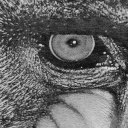
\includegraphics[width=0.9\textwidth]{reconstrucao/baboon_x2_viz.png}
        \caption{~\texttt{vizinho}.}
    \end{subfigure}%
    \hspace{8pt}
    \begin{subfigure}{0.3\textwidth}
        \centering
        \includegraphics[width=0.9\textwidth]{reconstrucao/baboon_x2_bil.png}
        \caption{~\texttt{bilinear}.}
    \end{subfigure}
    \\[8pt]
    \begin{subfigure}{0.3\textwidth}
        \centering
        \includegraphics[width=0.9\textwidth]{reconstrucao/baboon_x2_bic.png}
        \caption{~\texttt{bicubica}.}
    \end{subfigure}%
    \hspace{8pt}%
    \begin{subfigure}{0.3\textwidth}
        \centering
        \includegraphics[width=0.9\textwidth]{reconstrucao/baboon_x2_lag.png}
        \caption{~\texttt{lagrange}.}
    \end{subfigure}

    \caption{Escalonamento por um fator 2 seguido de outro escalonamento de fator 1/2 em \texttt{baboon128.png}, usando o mesmo método em cada caso.}
    \label{fig:rec:x2}
\end{figure}